From  \eqref{eq:solutions/13/11eq5},
\begin{align}
	\vec{V} = \myvec{1& \frac{5}{3} \\ \frac{5}{3} & 1}\label{myeq:solutions/13/11/}\\
	\vec{u}^T = \myvec{\frac{-5}{2} & \frac{-7}{2}}\label{df:solutions/13/11/}
\end{align}
and
\begin{align}\label{eq:solutions/13/11/dett}
\mydet{1& \frac{5}{3} & \frac{-5}{2} \\ \frac{5}{3} & 1 & \frac{-7}{2} \\ \frac{-5}{2} & \frac{-7}{2} & k} = 0 \\
\implies \brak{k - \brak{\frac{49}{4}}}-\frac{5}{3}\brak{\frac{5}{3}k - \frac{35}{4}} \nonumber\\
-
\frac{5}{2} \brak{\frac{-35}{6}+\frac{5}{2}} = 0\\
\implies \frac{64}k{36} - \frac{128}{12} = 0\\
\implies \boxed{k = 6} \label{eq:solutions/13/11result}
\end{align}
Substituting \eqref{eq:solutions/13/11result} in \eqref{eq:solutions/13/11eq5}, we get
\begin{align}
	x^{2}+ \frac{10}{3}(xy)+y^2 -5x -7y + 6 =0  \label{eq:solutions/13/11reseq}
\end{align}
Hence value of k=6 represents pair of straight lines.
Substituting value of k =6 in \eqref{eq:solutions/13/11/dett}
\begin{align}
\delta&=\begin{array}{|ccc|}
1 &\frac{5}{3}& \frac{-5}{2}\\\frac{5}{3} & 1 & \frac{-7}{2}\\ \frac{-5}{2} & \frac{-7}{2} & 6
\end{array}&
\intertext{Simplyfying  the above determinant , we get}
\delta&=0
\end{align}
%Since equation \eqref{eq:solutions/13/11det1} is satisfied, we could say that the given equation 
\eqref{eq:solutions/13/11reseq} represents two straight lines
\begin{align}
    \det(V)&=\begin{array}{|cc|}
1&\frac{5}{3}\\\frac{5}{3} & 1
\end{array}<0
\end{align}
Since $\det(V)<0$  lines would intersect each other
\begin{figure}[h]
    \centering
    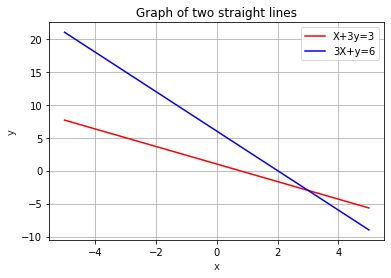
\includegraphics[width=\columnwidth]{./solutions/13/11/assignment5.png}
    \caption{Pair of straight lines}
    \label{Fig:solutions/13/11/1}
\end{figure}
%pair of straight lines in vector form is :
%\begin{align}
%    \vec{n_1}^T\vec{x}&=c_1\label{eq:solutions/13/11/m1}\\
%    \vec{n_2}^T\vec{x}&=c_2\label{eq:solutions/13/11/m2}
%\end{align}
%Equating their product with \eqref{eq:solutions/13/11eq4}
%\begin{align}
%(\vec{n_1}^T\vec{x}-c_1)(\vec{n_2}^T\vec{x}-c_2) &=\vec{x}^T\myvec{1 & \frac{5}{3} \\\frac{5}{3} & 1}\vec{x}\notag\\
%+2\myvec{\frac{-5}{2} & \frac{-7}{2}}\vec{x}+6\label{eq:solutions/13/11/86}
%\end{align}
\begin{align}
    \vec{n_1}*\vec{n_2}&=\{1,\frac{10}{3},1\}\label{eq:solutions/13/11/conv}\\
    c_2\vec{n_1}+c_1\vec{n_2}&=-2\myvec{\frac{-5}{2}\\\frac{-7}{2}}\label{eq:solutions/13/11/eq98}\\
    c_1c_2&=6
\end{align}
The slopes of the lines are given by the roots of the polynomial 
\begin{align}
    &cm^2+2bm+a=0\label{eq:solutions/13/11/e}\\
    \implies m_i&=\frac{-b\pm{\sqrt{-\det(V)}}}{c}\\
    \vec{n_i}&=k\myvec{-m_i\\1}
\end{align}
Substituting  in above equations \eqref{eq:solutions/13/11/e} we get,
\begin{align}
    &m^2+\frac{10}{3}m+1=0\\
    &\implies m_i=\frac{\frac{-10}{3}\pm{\sqrt{-(\frac{-16}{9})}}}{1}\label{eq:solutions/13/11/eq12}
\end{align}
Solving equation \eqref{eq:solutions/13/11/eq12} we have ,
\begin{align}
    m_1&=\frac{-1}{3}\\
    m_2&=-3\\
    \vec{n_1}&=k_1\myvec{\frac{1}{3}\\1}\label{eq:solutions/13/11/n1}\\
    \vec{n_2}&=k_2\myvec{{3}\\1}\label{eq:solutions/13/11/n2}
\end{align}
Substituting equations \eqref{eq:solutions/13/11/n1}, \eqref{eq:solutions/13/11/n2} in equation \eqref{eq:solutions/13/11/conv} we get 
\begin{align}
    k_1k_2&=1
\end{align}
Possible combination of ($k_1,k_2$) is (1,1)
Lets assume $k_1=1$, $k_2=1$, we get 
\begin{align}
    \vec{n_1}&=\myvec{\frac{1}{3} \\1}\label{eq:solutions/13/11/n11}\\
    \vec{n_2}&=\myvec{3\\1}\label{eq:solutions/13/11/n22}
\end{align}
we have:
\begin{align}
\vec{n_1}\ast \vec{n_2} = \myvec{a\\2b\\c} \label{eq:solutions/13/11conv1}
\end{align}
Convolution of $\vec{n_1}$ and $\vec{n_2}$ can be done by converting  $\vec{n_1}$ into a teoplitz matrix and multiplying with $\vec{n_2}$\\
From equation \eqref{eq:solutions/13/11/n11} and \eqref{eq:solutions/13/11/n22}
\begin{align}
    \vec{n_1}=\myvec{\frac{1}{3}&0\\1&\frac{1}{3}\\0&1}
    \vec{n_2}=\myvec{3\\ 1}\label{eq:solutions/13/11conv2}\\
\implies \myvec{\frac{1}{3}&0\\1&\frac{1}{3}\\0&1}\myvec{3\\ 1} = \myvec{1\\\frac{10}{3}\\1} = \myvec{a\\2b\\c}\label{eq:solutions/13/11conv3}
\end{align}
$c_1$ and $c_2$ can be obtained as,
\begin{align}
\myvec{\vec{n_1} & \vec{n_2}}\myvec{c_2\\c_1}&=-2\vec{u}\\
\myvec{\vec{n_1} & \vec{n_2}}\myvec{c_2\\c_1}&=-2\myvec{\frac{-5}{2}\\\frac{-7}{2}}
\label{eq:solutions/13/11aug1}
\end{align}
Substituting \eqref{eq:solutions/13/11/n11} and \eqref{eq:solutions/13/11/n22} in \eqref{eq:solutions/13/11aug1}, the augmented matrix is,
\begin{align}
\myvec{\frac{1}{3} & 3& 5 \\ 1 & 1 & 7}
\xleftrightarrow[]{R_1 \leftarrow 3\times R_1}
\myvec{1 & 9&15\\ 1 & 1 & 7}
\end{align}
\begin{align}
\myvec{1 & 9&15\\ 1 & 1 & 7}
\xleftrightarrow[]{R_2 \leftarrow R_2- R_1}
\myvec{1 & 9&15\\ 0 & -8 & -8}
\end{align}
\begin{align}
\myvec{1 & 9&15\\ 0 & -8 & -8}
\xleftrightarrow[]{R_2 \leftarrow R_2\div -8}
\myvec{1 & 9&15\\ 0 & 1 & 1}
\end{align}
\begin{align}
\myvec{1 & 9&15\\ 0 & 1 & 1}
\xleftrightarrow[]{R_1 \leftarrow R_1-9\times R_2}
\myvec{1 & 0&6\\ 0 & 1&1 }
\end{align}
From above  we get 
\begin{align}
    c_1&=1\\
    c_2&=6
\end{align}
Hence pair of straight lines  are
%from  \eqref{eq:solutions/13/11/m1}, \eqref{eq:solutions/13/11/m2} in vector form
\begin{align}
    \myvec{\frac{1}{3}& 1}\vec{x}&=1\\
    \myvec{3 & 1}\vec{x}&=6
\end{align}

   
